\documentclass[12pt,a4paper]{article}
\usepackage[textheight=28cm,textwidth=19cm,headheight=10mm,footskip=10mm]{geometry}
\usepackage[UTF8]{inputenc}
\usepackage[T1]{fontenc}
\usepackage[french]{babel}
\usepackage{fourier}
\usepackage{amsmath,amsfonts,amssymb}
\usepackage{paralist,array}
\usepackage{pgf,tikz}
\usetikzlibrary{shapes,snakes,arrows}
\usepackage{graphicx,multicol,varwidth}
\usepackage{pstricks-add}

\pagestyle{empty}

\newcommand{\ent}[4]{\begin{flushleft}
\underline{#1}
\hfill
\underline{#2$^{\text{ème}}$ #3}
\vspace{12 pt}
\end{flushleft}
\begin{center}
\begin{LARGE}
\textbf{\underline{\'Evaluation sur Scratch n°#4}}
\vspace{12 pt}
\end{LARGE}
\end{center}}
%fin de la commande \ent (entête du contrôle)

\renewcommand{\arraystretch}{1.5}

\begin{document}
\ent{\textit{date à mettre}}{3}{}{1}
\begin{enumerate} [1{)}]
\item
Tracer, à main levée et à côté du script ci-dessous, la figure que scratchy trace. \vspace{3pt} \\
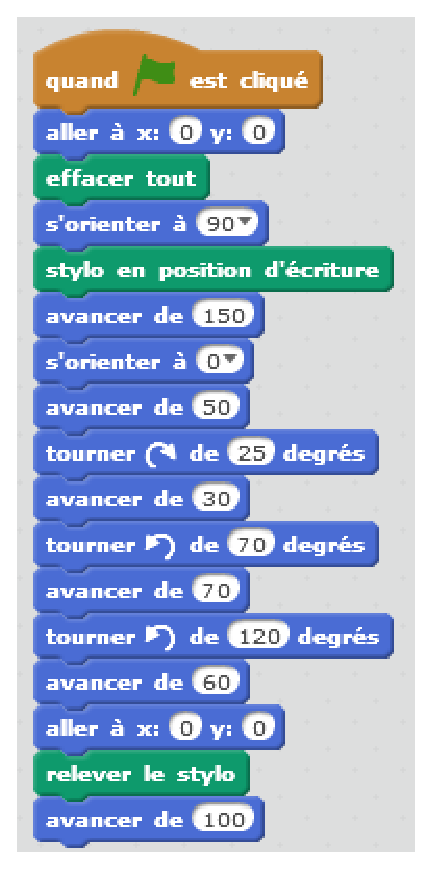
\includegraphics[scale=0.5]{Evaluation1_Script.eps} \vspace{3pt}
\item
Coder votre figure. \vspace{3pt}
\item
\begin{enumerate} [a{)}]
\item
Qu'est qu'un élément déclencheur ? \, \dotfill \vspace{9pt} \\
.\dotfill \vspace{9pt}
\item
Quel est l'élément déclencheur de ce script ? \dotfill  \vspace{9pt} \\
\end{enumerate}
\item
Que fait l'instruction 
\includegraphics[scale=0.5]{Evaluation1_a.eps} ? \dotfill  \vspace{9pt} \\
.\dotfill \vspace{9pt} \\
\item
Que permet de faire les deux dernières instructions ? \dotfill  \vspace{9pt} \\
.\dotfill \vspace{9pt} \\
\end{enumerate}
\vfill
NOM - Prénom : \dotfill 

\end{document}